\section{Memory and Addressing Modes}
\subsection{Memory}
Memory is an incredibly important component of a computing system:
\begin{itemize}
    \item We store our \important{programs} in it 
    \item We store our \important{data} in it 
	\item It is often through memory that we will \important{receive data and send out data}
\end{itemize}
	Memory is a reccurent ropic in this course, we have already seen it with the stack however the type of the memory is also an important topic:
	\begin{itemize}
		\item Memory can be \important{very slow} $\implies $ Caches 
		\item Memory is \textit{finite} (relatively small) $\implies $ Virtual memory 
		\item Memory can make an \important{ISA too complex} $\implies $ pipelining
	\end{itemize}
	\paragraph{Types of memory}
	There is a lot of different technologies for memory:
	\begin{itemize}
		\item SRAM, DRAM, EPROM, Flash, etc.
\end{itemize}
Each of those has a variations in \important{capabilities} therefore also in how we use them, memory change by:
\begin{itemize}
	\item Capacity, density 
	\item Speed 
	\item Writable, permanent, reprogrammable
\end{itemize}
\begin{center}
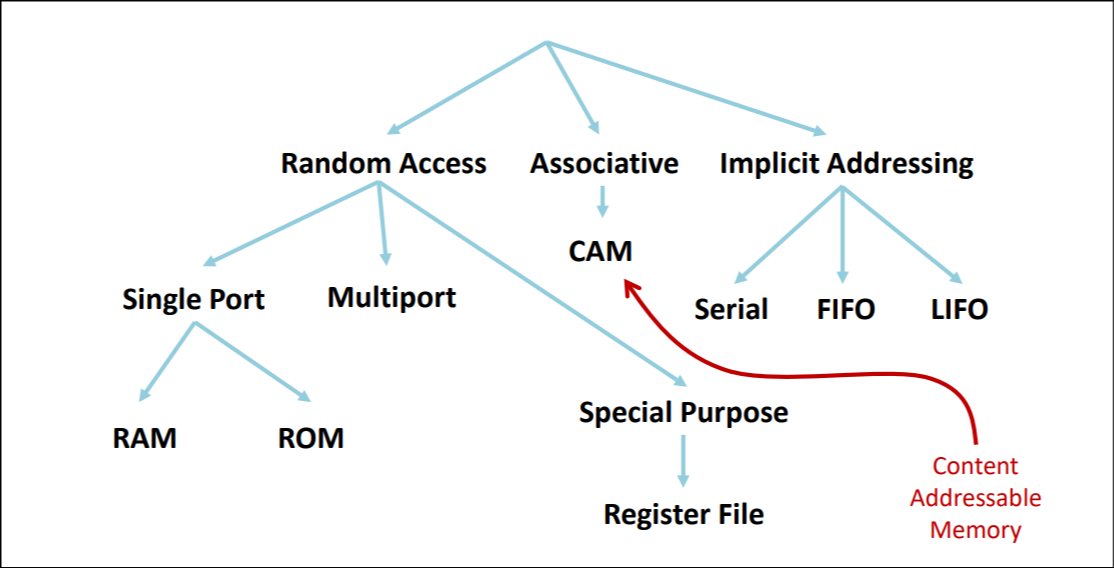
\includegraphics[scale=0.4]{screenshots/2025-10-11_8.png}
\end{center}
We have here all the type of memory that can be used, What we use when we program are Random access memory, this means that the memory can be accessed with an address. In the tree of random access memory we have:
\begin{center}
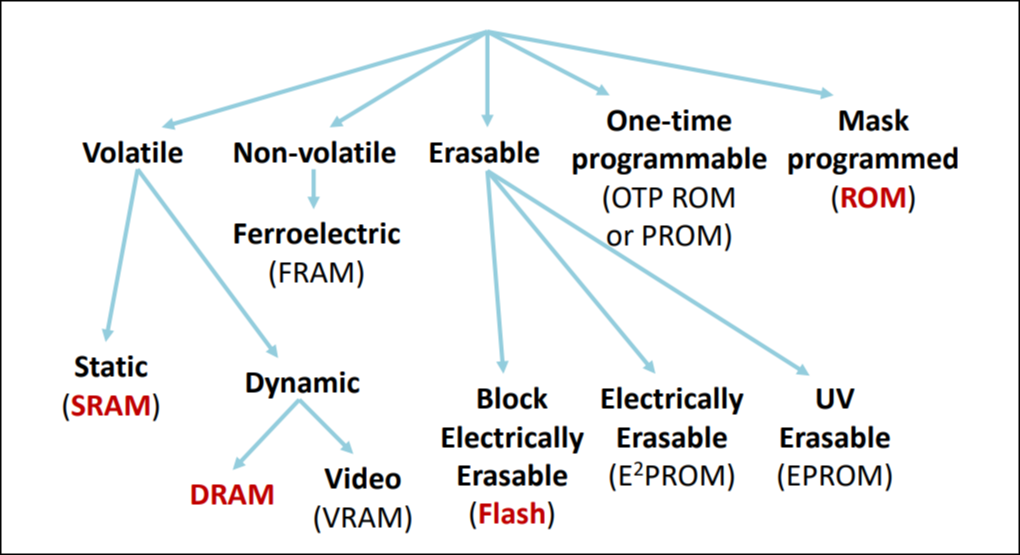
\includegraphics[scale=0.4]{screenshots/2025-10-11_9.png}
\end{center}
The basic structure behind those memory are DFF, (D flip flop). which are stacked one on another in a $n$ times 4 grid. Each flip flop looks like this:
\paragraph{SRAM}
SRAM stands for \important{static random access memory}. It sores data with flips flops which makes it faster than DRAM (which we will see later) but more expensive. We use it for CPU caches and for the register file
\begin{center}
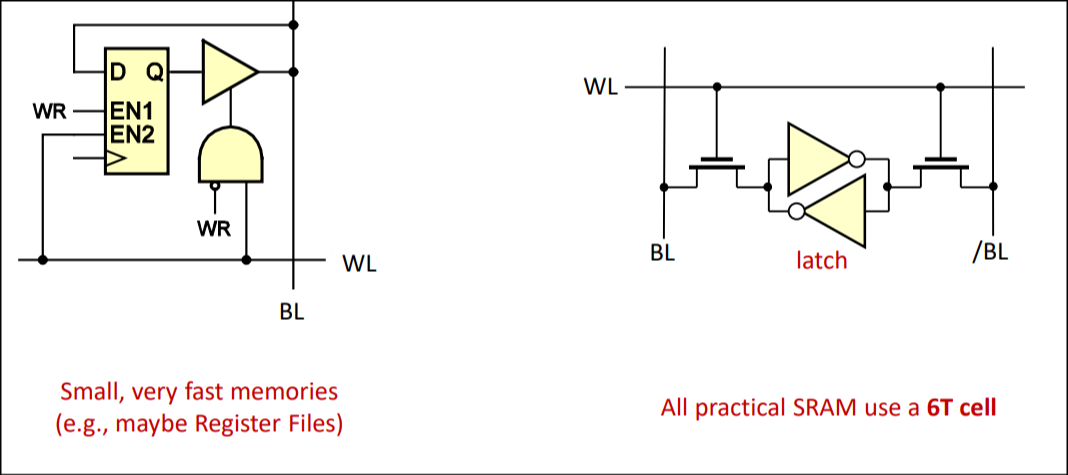
\includegraphics[scale=0.3]{screenshots/2025-10-11_10.png}
\end{center}
So here we have to make a difference between the boolean system and the electrical components. The circuit on the left is a desastre in term of electrical components it has approximatevely 20 transistors which makes it \important{slower} \textbf{and} \important{costlier}. The real way to do SRAM is with the right circuit. However this looks bad, normally it is forbidden to have a closed loop in a circuit! We are forbidden to have a loop in our circuit without a flip flop in it, you cannot have a loop inside a combinational circuit. So this is a big special thing for us however, this "works", it is compatible there is no issue in the circuit. The issue we have is that:\\
Imagine putting a one on the left or right part of the circuit $\implies$ the value cannot be changed, it is stucked there for ever. This looks really good because one \textbf{NOT} gate costs us only two transistors so the memory (loop) costs us only 4 transistors. But we still need to write and read from the memory, to do so we had the two transistors (see on the image) which also us to let the memory live on its own (when the transistors are open) \textbf{or} to be connected to the world. \\
If I want to see what is on the memory I put one in the word line (WL) and I will get the value on the bit line.\\
The question now is how to write? As said earlier, now we have a signal that is stored in there but it is stored for infinity.\\
The only way to write is to "\textit{shout louder than the current signal}".  Imagine we currently have a 1 as the output of the latch and I want to put a 0. If I shout 0 louder than the 1 while connected, it will have a short circuit... and this is bad. \textbf{However} what is going on in fact is the upper not gate will have two inputs, a \textbf{loud} 0 and a quiet 1, the not fate will then take the loudest one thus 0.\\
And now it will take a really short time to the latch to adapt itself to the new value, the short circuit here take the times two the 0 to go trhough two not gates. and then it agrees.\\

On the other hand we have DRAM:
\paragraph{DRAM}
\begin{itemize}
    \item  Dynamic RAMs are the densest (and thus cheapest) form of random access semiconductor memory 
    \item DRAMs store \important{information as charge in small capacitors} part of the memory cell 
    \item First parented in 1968 by Robert Dennard, scaled amazingly over decades and was somehow an important ingredient of the progress of computing systems.
    \item charges \important{leaks off} the capacitors due to parasitic resistance $\implies $ every DRAM cell needs a \important{periodic refresh} (e.g. every \~60ms) lest it forgets information.
\end{itemize}
So imagine, if we don't go in each cell every 60ms then we lose the information, but we have other things to do? So how do we do it? - we have someone else refresh them for us. The memory controller is reponsible for refreshing the contents of the DRAM instead of the CPU.
\begin{center}
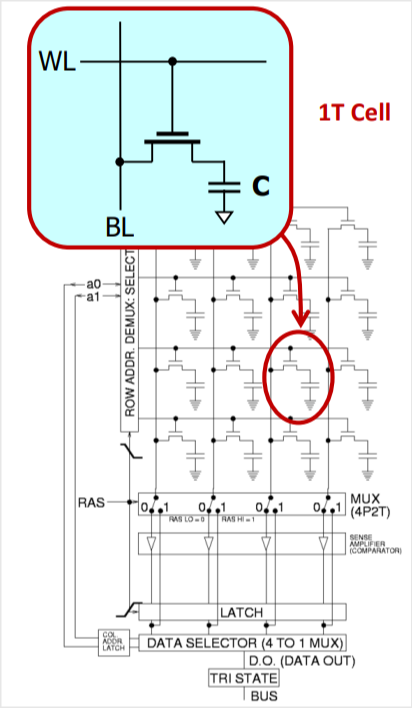
\includegraphics[scale=0.3]{screenshots/2025-10-12.png}
\end{center}
The goal after this is to access those memory celle based on the address we input. The \textit{ideal} way to do so, would be to have one \textbf{big} decoder that treats the adress and directly output the information in the memory celle like this:
\begin{center}
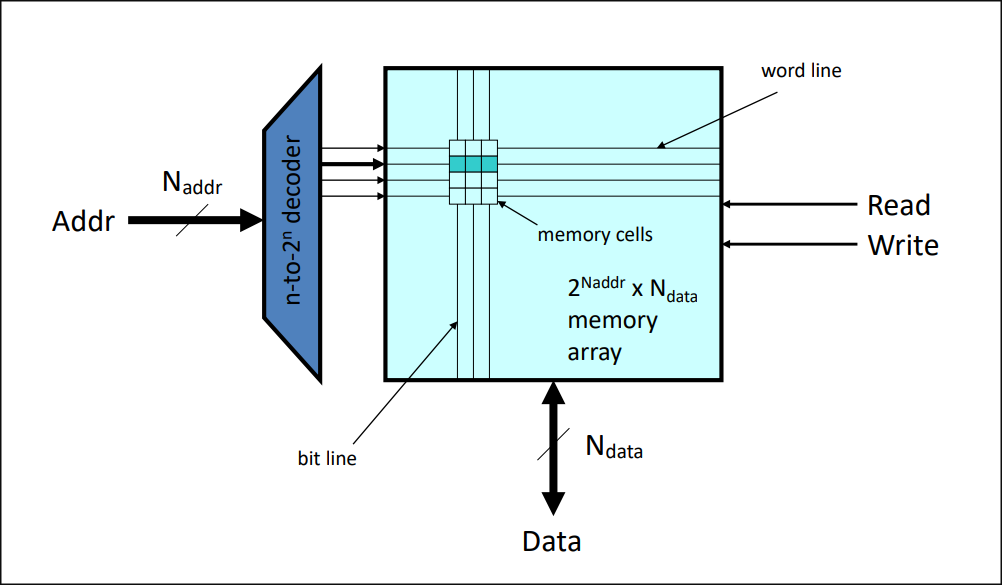
\includegraphics[scale=0.2]{screenshots/2025-10-12_1.png}
\end{center}
However life is not always that easy, and there is a lot of way to get the memory celle based on the address, here are some example:
\begin{center}
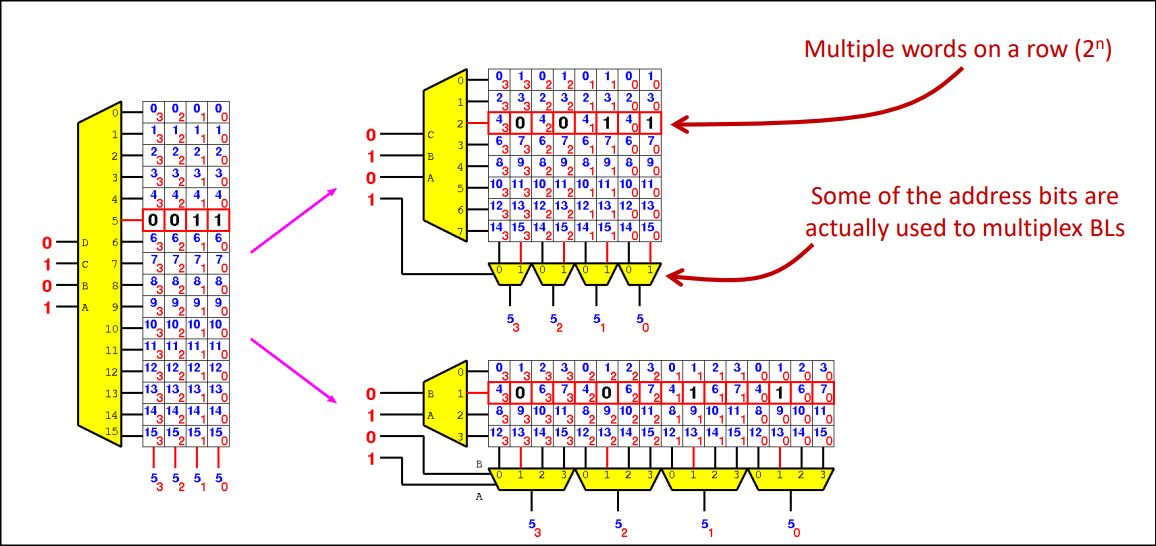
\includegraphics[scale=0.4]{screenshots/2025-10-12_2.png}
\end{center}
Here we have 3 ways to do so:
\begin{itemize}
    \item On the left, We have the same way as the \textit{ideal} decoder with one byte per row 
    \item However we can also split up into a grid with more than one \textbf{big} multiplexer. This implies that there will be multiple word by row and that the bytes are not necesserly ordered.
\end{itemize}
The best physical way to create a Random access memory is in a square to minimize parasitic capacitance of BL (bit line) and WL (word line). We want to having it into the most squared possible form because:
\begin{itemize}
	\item When a word line is activated (row), the bit line carries the data (bit) stored in the selected memory cell to the output circuitry (like a multiplexer or sense amplifier).
	\item Activating a word line selects all the bits (across bit lines) in that row — this is your selected "word."
\end{itemize}
Therefore by having the smallest length, we get shorter lines $\implies $ lower parasitic capacitance $\implies$ faster access, lower power, and more reliable operation.
\begin{center}
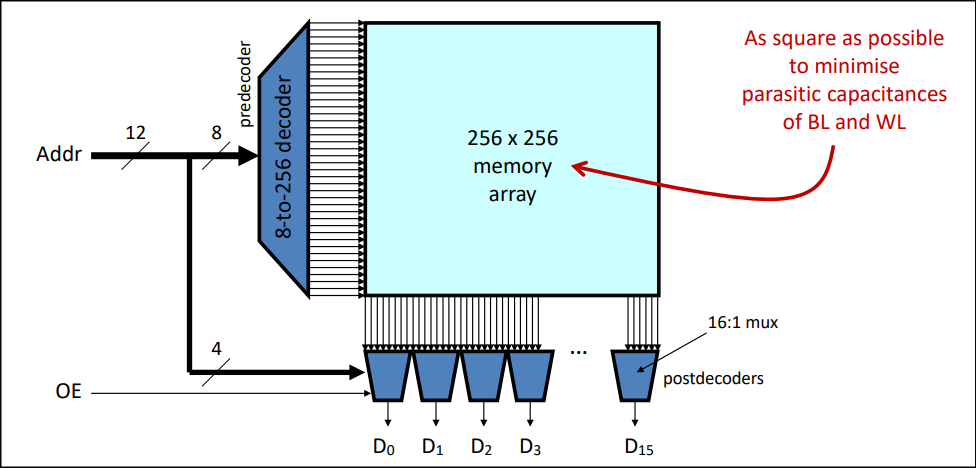
\includegraphics[scale=0.3]{screenshots/2025-10-12_3.png}
\end{center}

\begin{framedremark}

Every time we are looking for a memory cell, we need to charge all row and then all column, the goal here is to minimize the number $x =r + c$ by a fixed area $A$ (where $A$ is the number of cell):\\
We have that
\begin{align*} A = rc \\
				\frac{A}{c} = r
\end{align*}
Which implies that $x = \frac{A}{c} + c$, we are minimizing  ($x' = 0$) this:
\begin{align*} 
	x' = -\frac{A}{c^2} + 1 \\
	\frac{A}{c^2} = 1 \\
	c^2 =  A \implies c = \sqrt{A}
\end{align*}
And because we know that $A =  rc \implies r =  c =  \sqrt{A}$ which is a square.

\end{framedremark}
\paragraph{Static RAM typical interface}
This is the typical synchronous SRAM that we have already seen before:
\begin{center}
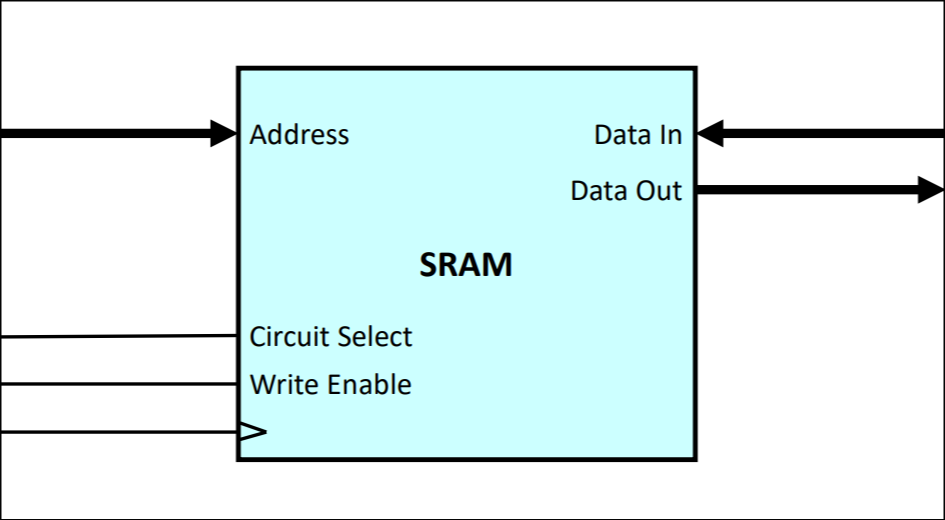
\includegraphics[scale=0.2]{screenshots/2025-10-12_4.png}
\end{center}
However we don't always has to be synchronous, we can also be asynchronous for a Read cycle which works like this:
\begin{parag}{Asynchronous read cycle}
    

\begin{itemize}
    \item Enable the memory $\to$ assert the address $\to $ wait for the data 
		\begin{itemize}
		    \item Data out is available after a combinational delay $T_{acc} = $ Access Time 
		\end{itemize}
		\item Maximum frequency is limited by the minimum $T_{cyc}$ (time for a cycle, time for us to be able to change the address)
\end{itemize}

\begin{center}
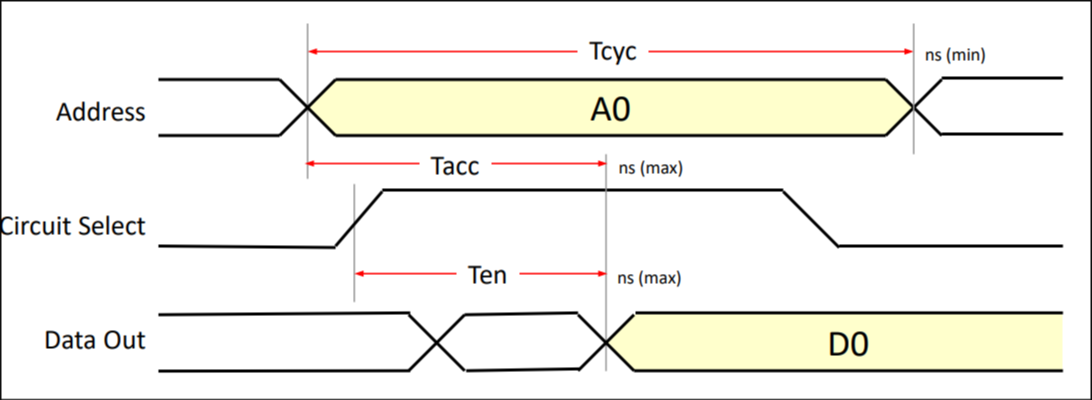
\includegraphics[scale=0.25]{screenshots/2025-10-12_6.png}
\end{center}

\end{parag}
\begin{parag}{synchronous SRAM Read cycle}
    

Here this is the other way around, we always wait a rising edge of the clock to do anything. Everything here is working like a flip flop:
\begin{itemize}
    \item Everything is relative to the clock signal
    \item Latency is the number of cycles between the address asserted and data available
		\begin{itemize}
			\item Often one as in this diagram but in some cases (large memories) more
		\end{itemize}
\end{itemize}


\begin{center}
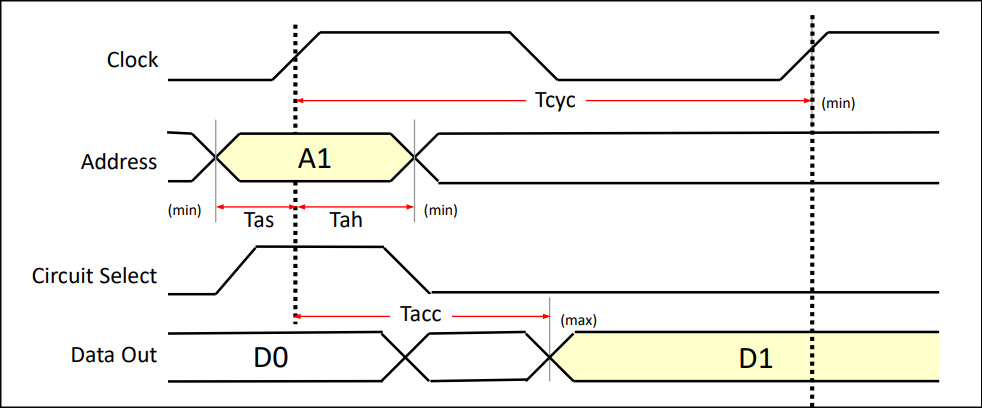
\includegraphics[scale=0.25]{screenshots/2025-10-12_7.png}
\end{center}
\end{parag}
\subsubsection{Load and store instrucitons}
Now that we have seen how it works, we want to see how to implement a load from the memory into the register file. For instance the following intrsuction:
\begin{lstlisting}[language={[RISC-V]Assembler}]
lw x5, (123456)
\end{lstlisting}
This is not a RISC-V instruction but bear with us. (I am not sure that's a saying...)


\begin{center}
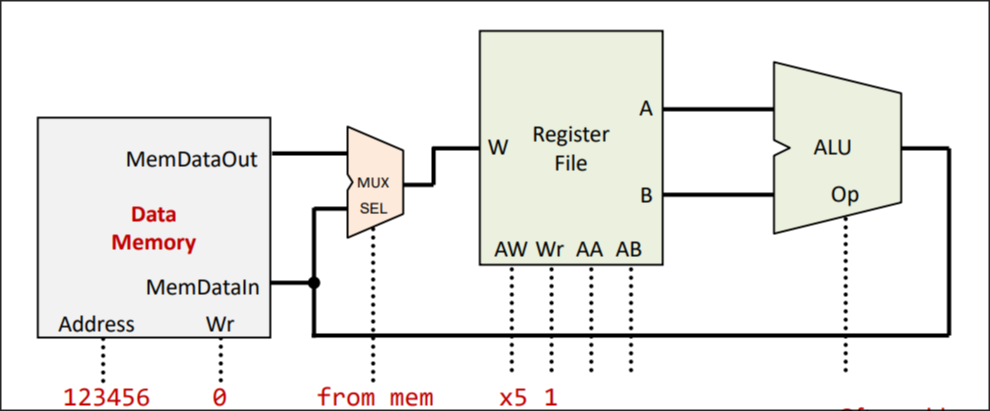
\includegraphics[scale=0.3]{screenshots/2025-10-12_8.png}
\end{center}
What we have changed here is the left part now instead of having a loop like $\text{ALU} \to \text{Register file} \to \text{ALU}$ we break it at the first "$\to$" and add a multiplexer there to be able to interact with the memory. \\

For the store instruction, instead of using the \texttt{MemDataOut} path, we use the \texttt{MemDataIn}.\\
The main diffrence is this:
\begin{center}
    


\begin{tikzpicture}[
    block/.style = {draw, minimum width=2.4cm, minimum height=1cm, align=center},
    arrow/.style = {thick, -{Latex}},
    node distance=1.8cm and 1.8cm
]

%% LOAD PATH

\node[block] (regfileL) {Register File\\(base)};
\node[block, right=of regfileL] (aluL) {ALU\\(base + offset)};
\node[block, right=of aluL] (memL) {Memory};
\node[block, right=of memL] (outregL) {Register File\\(destination)};

\draw[arrow] (regfileL) -- (aluL);
\draw[arrow] (aluL) -- (memL);
\draw[arrow] (memL) -- node[above]{\scriptsize{MemDataOut}} (outregL);

\node[above=0.5cm of aluL] {Load Instruction};

%% STORE PATH

\node[block, below=2.5cm of regfileL] (regfileS1) {Register File\\(base)};
\node[block, right=of regfileS1] (aluS) {ALU\\(base + offset)};
\node[block, right=of aluS] (memS) {Memory};

\node[block, below=1.5cm of aluS] (regfileS2) {Register File\\(value)};
\draw[arrow] (regfileS1) -- (aluS);
\draw[arrow] (aluS) -- (memS);
\draw[arrow] (regfileS2) -- node[right]{MemDataIn} (memS);

\node[above=0.5cm of aluS] {Store Instruction};

\end{tikzpicture}
\end{center}
\begin{framedremark}
	I had some trouble understand how does the value just pop, but if I understand it right, the register value is stored from the register file into \texttt{B} here. We use the \texttt{A} port as a address base. This is how it works:
\begin{enumerate}
    \item IF, Fetch instruction ( \texttt{sw x2, 8(x1)})
    \item ID, Read \texttt{x1} and \texttt{x2} from register file 
    \item EX, ALU compute \texttt{x1 + 8} (address) 
    \item MEM, Store \texttt{x2} to memory at computed address 
    \item WB, Nothing (no register to write for store)
\end{enumerate}
\end{framedremark}

\paragraph{Why RISC-V instructions are so simple?}%
\label{par:Why RISC-V instructions are so simple?}

\begin{framedremark}
Here are some example of some instruction that would look correct in RISC-V but is not (for addition):
\begin{itemize}
    \item Based or Indexed
		\begin{lstlisting}[language={[RISC-V]Assembler}]
	add x0, x1, i5(x2)		#x0 = x1 + mem[x2 + i5]
		\end{lstlisting}
	\item Auto-increment or -decrement
		\begin{lstlisting}[language={[RISC-V]Assembler}]
	add x0, x1, (x2+) 		#x0 = x1 + mem[x2]
		\end{lstlisting}
	\item PC-relative
		\begin{lstlisting}[language={[RISC-V]Assembler}]
	add x0, x1, 123(pc)		#x0 = x1 + mem[pc + 123]
		\end{lstlisting}
\end{itemize}
However those instruciton \important{does not exist} in RISC-V.\\
RISC-V is designed to have  two world: one for accessing memory, and one for the logic/arithmetic etc. We cannot mix them together.\\
However in x86/x64 we can do this:
\begin{lstlisting}[language={[x64]Assembler}]
	ADD DWORD PTR [EBX + ESI*4 + 16], EAX
\end{lstlisting}
This means:
\begin{itemize}
    \item The \texttt{DWORD} means double word which means that we are working on 64 bits number.
	\item The \texttt{ADD} that has only two operand, the reason why, is that the goal of x86 in 1979 was to be the most compact possible, at that time the memory was limited and to be able to write program you had to be careful of the size of the program that you are writing. So they added the constraints that the output of the instruction is stored in the first operand. \\ this means we take something in the memory at \texttt{[EBX + ESI*4 + 16]}, add it with \texttt{EAX} and then store it in \texttt{[EBX + ESI*4 + 16]}. 
\end{itemize}
	 this feels pretty slow and pretty confusing, just try to map this into the CPU we created before, this would look like this:
		\begin{center}
		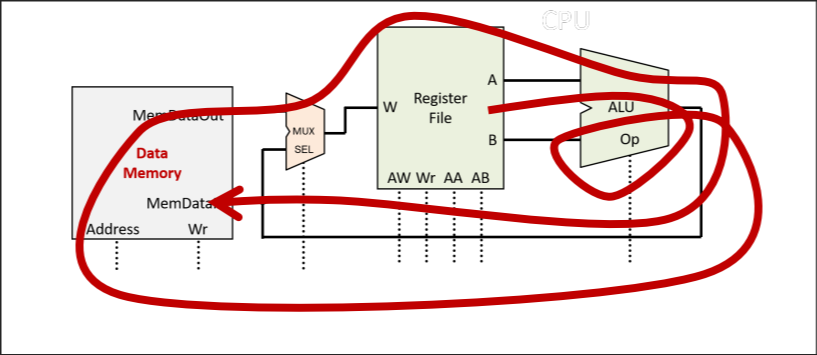
\includegraphics[scale=0.2]{screenshots/2025-10-12_9.png}
		\end{center}
We would need to go like four times to the ALU, the fact is that \important{this is possible} however it makes it hard to optimize the processor.
\end{framedremark}
The question behind all this is how does intel can still be as famous as they are now with instruction that looks like this and that cannot really be optimized? There is still the majority of the processor to this day that are intel processor (even if amd is better...), we will see this in a couples of weeks.
\subsubsection{Byte addressed memory}

Almost all ISA today are use byte addressed memory. byte are quite important, disks are organized in bytes, network packets are bytes, \important{ascii} are byte. A lot of data are represented as byte so using an word addressed memory wouldn't be very efficient here, we would either loose a lot of time looking for the right byte, or loosing a lot of space by putting byte in word address (losing the three other bytes).\\
The solution is to no change the way memory is placed \textbf{but} \important{changing the label}.
\begin{center}
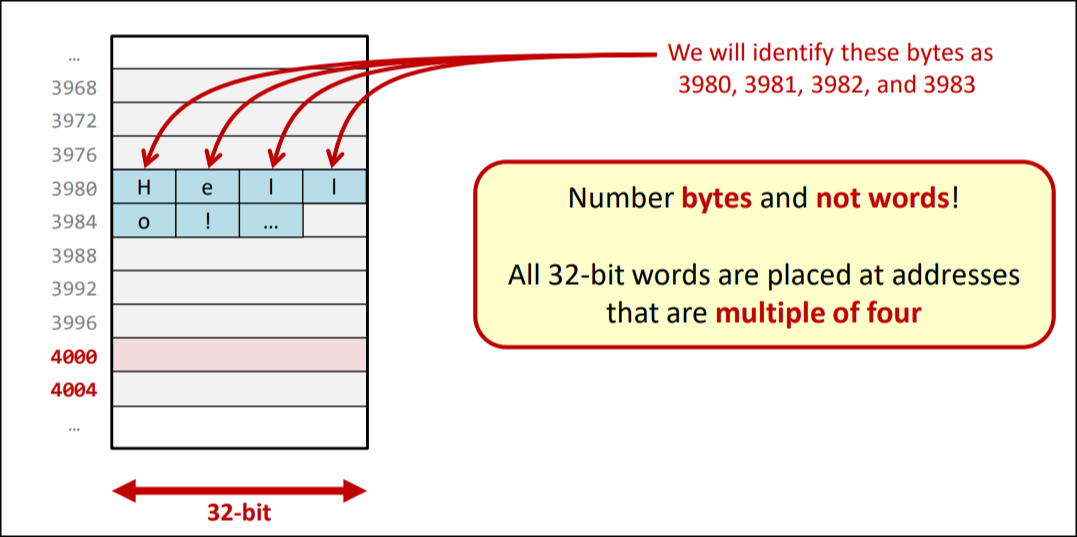
\includegraphics[scale=0.3]{screenshots/2025-10-12_10.png}
\end{center}
\paragraph{Loading a word (\texttt{lw}) and Instruction}%
For instance, if we are interested in word, we cannot look for the word at address 3981, this would'nt be a word.
\begin{center}
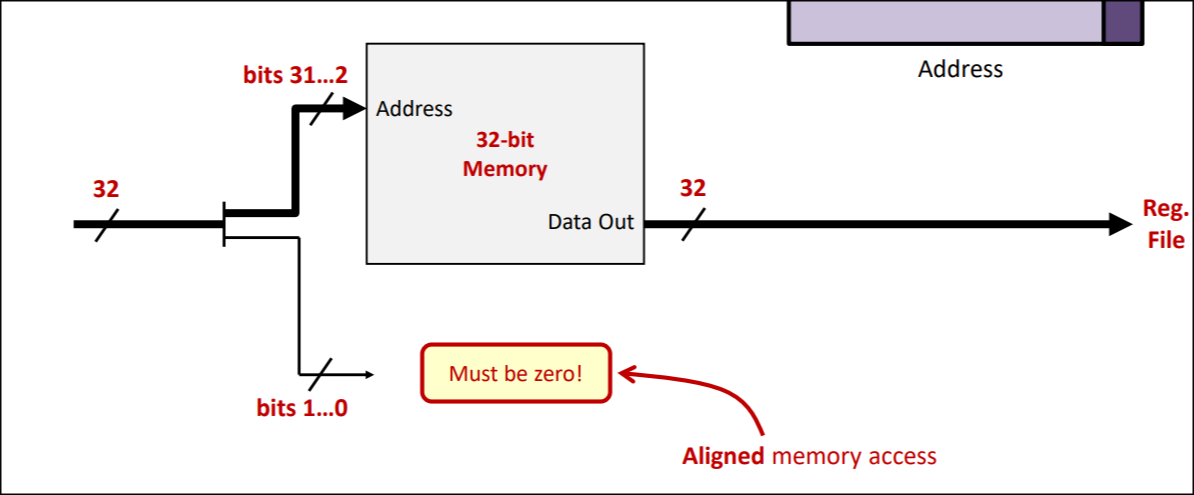
\includegraphics[scale=0.25]{screenshots/2025-10-12_11.png}
\end{center}
As said before when loading a word, it has to be a multiple of 4 so we only care about the 30 most significant bits. The two least significant bits is checked wether there are zero or not and if there are not zero, we would like to \important{throw an exception} which we will see how in a couple of weeks.

\paragraph{Loading byes (\texttt{lb})}%
Here what we are doing is the same as what we did before, we are looking for a word (which is the 30 first bits), and then in the word we choose which 8 bits we wants, this would look like this:
\begin{center}
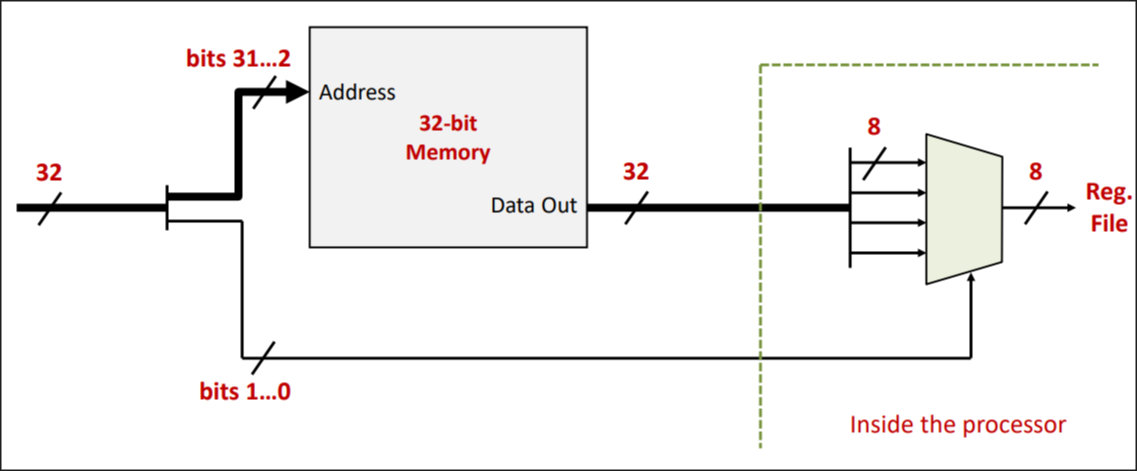
\includegraphics[scale=0.25]{screenshots/2025-10-12_12.png}
\end{center}

Remember when we changed the shape of the memory, how we choose which bit to take; we are doing  the \important{same} here too. The difference is that this part is only in the processor, circuit wise this change nothing.\\
What is good here is that by just adding a multiplexer we can add a lot of instruction in the ISA.
